% !TeX spellcheck = en_US
\documentclass[letterpaper,12pt,twoside]{report}
\usepackage{fancyhdr}
\usepackage{fullpage}
\usepackage{tikz}
\usepackage{textcomp}
\usepackage{amsmath}

\begin{document}
	\pagestyle{fancy}
	\fancyhf{}
	\fancyhead[L]{Day 7}
	\fancyhead[R]{\textit{The Calendar Project}}
	\fancyfoot[L]{Citations Involved: none}
	
	% Problem
	\paragraph{Problem}
	\begin{quote}
	\textsf{\textrm{\textit{GUIDANCE}} is a regular octagon
		with center $O$. We define $R_1$, $R_2$, and $R_3$
		as counter-clockwise rotations of, respectively, 45\textdegree, 90\textdegree, and 135\textdegree \space about $O$. Which diagonal will be mapped onto $\overline{CI}$ if each rotation is applied exactly once?}
	\end{quote}
	
	% Graphics
	\begin{center}
		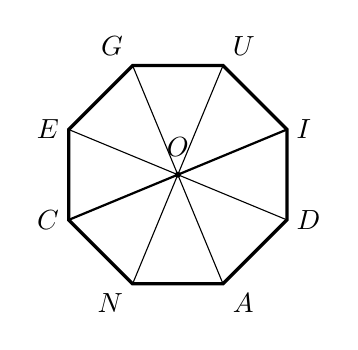
\begin{tikzpicture}[scale=1.5]
		\draw[very thick] (0.92388,0.3827) -- (0.92388,-0.3827) -- (0.3827,-0.92388) -- (-0.3827,-0.92388) -- (-0.92388,-0.3827) -- (-0.92388,0.3827) -- (-0.3827,0.92388) -- (0.3827,0.92388) -- cycle;
		
		\node[above left] at (-0.3827,0.92388) {$G$};
		\node[above right] at (0.3827,0.92388) {$U$};
		\node[right] at (0.92388,0.3827) {$I$};
		\node[right] at (0.92388,-0.3827) {$D$};
		\node[below right] at (0.3827,-0.92388) {$A$};
		\node[below left] at (-0.3827,-0.92388) {$N$};
		\node[left] at (-0.92388,-0.3827) {$C$};
		\node[left] at (-0.92388,0.3827) {$E$};
		
		\draw[fill=black] (0,0) circle [radius=0.02];
		\node[above] at (0,0.07) {$O$};
		
		\draw (0,0) -- (-0.92388,0.3827);
		\draw[thick] (0,0) -- (-0.92388,-0.3827);
		\draw (0,0) -- (-0.3827,-0.92388);
		\draw (0,0) -- (0.3827,-0.92388);
		\draw (0,0) -- (0.92388,-0.3827);
		\draw[thick] (0,0) -- (0.92388,0.3827);
		\draw (0,0) -- (0.3827,0.92388);
		\draw (0,0) -- (-0.3827,0.92388);
		
		\end{tikzpicture}
	\end{center}
	
	% Reasoning
	\paragraph{Reasoning}
	\begin{quotation}
	
	It can be deduced from the Angle Addition Postulate (1) that Euclidean rotation angles are accumulative (i.e. two 45\textdegree \space rotations $\equiv$ one 90\textdegree \space rotation), which means that applying all of the given rotation angles exactly once is equivalent to \textbf{one} $45+90+135=270$\textdegree \space counter-clockwise rotation. This is equivalent to one $360-270=90$\textdegree \space clockwise rotation because one full rotation is $360$\textdegree. Given that \textit{GUIDANCE} is a regular octagon, the 8 segments connecting its center to its vertices divide the full rotation around its center into 8 central angles (i.e. $\angle NOA$). Since each central angle of a regular $n$-gon has a measure of $\frac{360\textdegree}{n}$, their measures in $GUIDANCE$ are equal to $\frac{360}{8}=45$\textdegree. Coincidentally, the deduced angle of the rotation to be performed has a measure of $45\cdot2=90$\textdegree, indicating that each vertex will map onto one that is $\frac{90}{45}=2$ sides away (i.e. $D$ to $U$). Making a $90$\textdegree \space counter-clockwise rotation from $\overline{CI}$ determines the  diagonal that would map onto its position after the $90$\textdegree \space clockwise rotation; after such application, $\overline{CI}$ maps onto $\boxed{\overline{AG}}$, which is the solution to this problem.
	
	\end{quotation}
	
	\iffalse
	
	\paragraph{External References}
	
	\begin{enumerate}
		\item Textbook Ch. 9, Pg. 589: Area of Parallelograms
		\item Textbook Ch. 9, Pg. 590: Area of Triangles and Trapezoids
	\end{enumerate}
	\fi

\end{document}